\documentclass[a4paper,12pt]{article}
\usepackage[utf8]{inputenc}
\usepackage[italian]{babel}
\usepackage{amsfonts}
\usepackage{listings}
\usepackage{xcolor}
\usepackage{booktabs}
\usepackage{graphicx}
\usepackage{float}
\setcounter{tocdepth}{4}
\setcounter{secnumdepth}{4}

\title{Maps}
\author{Appunti di Programmazione}
\date{\today}

\begin{document}
\tableofcontents
\newpage

\maketitle

\section{MultiWay Search Trees \& B-Trees}

\subsection{Multiway Search Tree}
\begin{figure}[H]
    \centering
    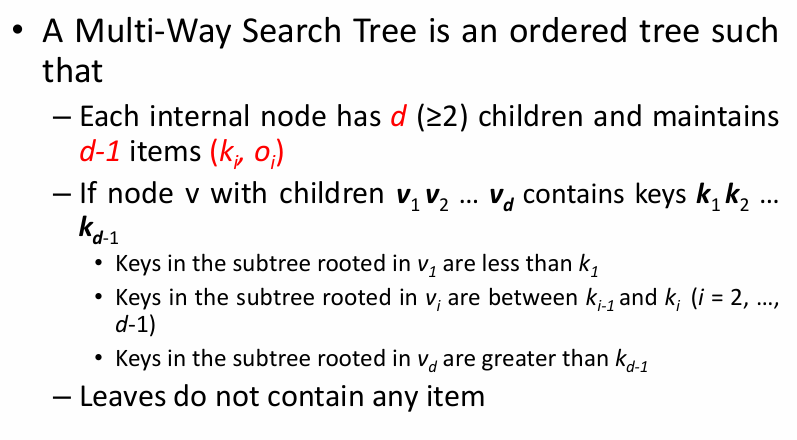
\includegraphics[width=0.47\linewidth]{Immagini/MWSTdef.png}
    \vline
    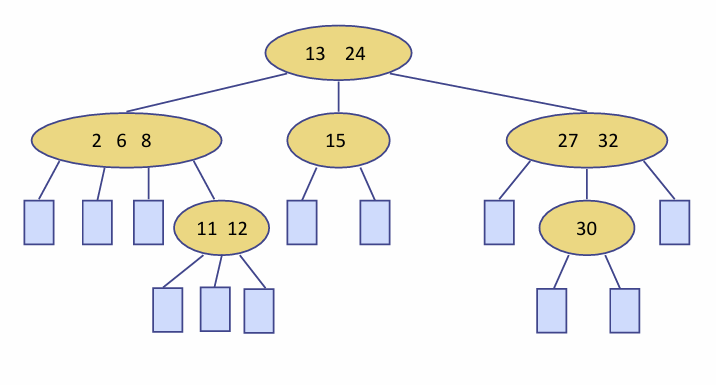
\includegraphics[width=0.47\linewidth]{Immagini/MWSTExample.png}
    \caption{MultiWay Tree}
\end{figure}

\subsubsection{Useful Property}
\begin{figure}[H]
    \centering
    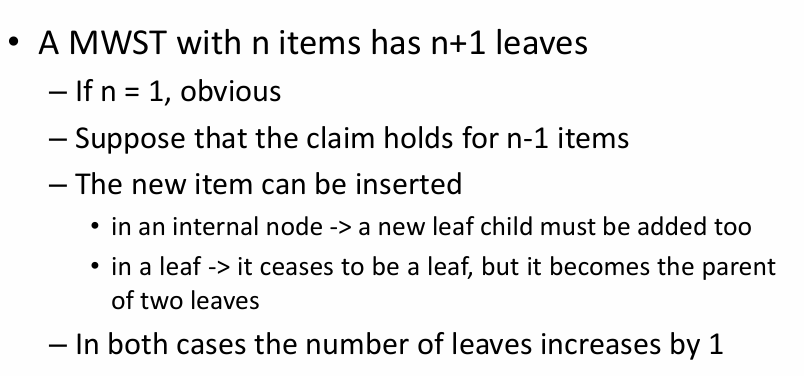
\includegraphics[width=0.47\linewidth]{Immagini/MWSTproperty.png}
    \caption{Useful Property}
\end{figure}

\subsection{a-bTree}
A differenza degli alberi binari, dove ogni nodo ha al massimo 2 figli, qui ogni nodo può averne molti di più, rendendo l'albero molto più "basso" e largo.
\textit{Perché se b è pari, allora: $$2 \le a \le b/2 $$ mentre se b è dispari, allora:  $$2 \le a \le (b-1)/2$$???}

Serve a garantire che, dopo una divisione, entrambi i nuovi nodi abbiano almeno $a$ figli. 
\begin{itemize}
    \item \textbf{Se $b$ è pari (es. $b=6$)} :Dividendo $b+1$ figli (cioè 7), ottieni $\lfloor 7/2 \rfloor = 3$ e $\lceil 7/2 \rceil = 4$. Per far sì che entrambi siano validi, 
          il minimo $a$ deve essere al massimo 3. ($b/2$).
    \item \textbf{Se $b$ è dispari (es. $b=5$)}: Dividendo $b+1$ figli (cioè 6), ottieni $6/2 = 3$ e $3$. Il minimo $a$ deve essere al massimo 3.
          $((b+1)/2$, che è coerente con la formula $(b-1)/2$ se consideri il numero di chiavi invece dei figli).
\end{itemize}

\begin{figure}[H]
    \centering
    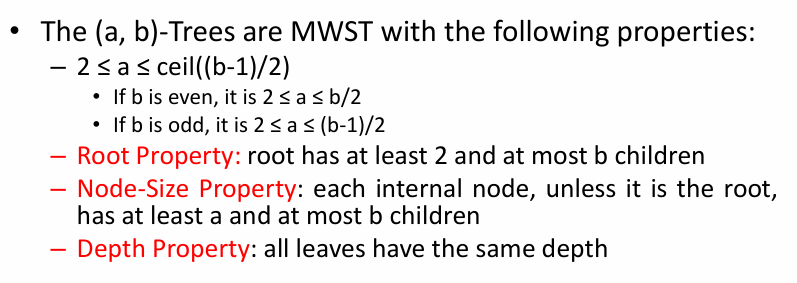
\includegraphics[width=0.47\linewidth]{Immagini/abTreeDef.png}
    \vline
    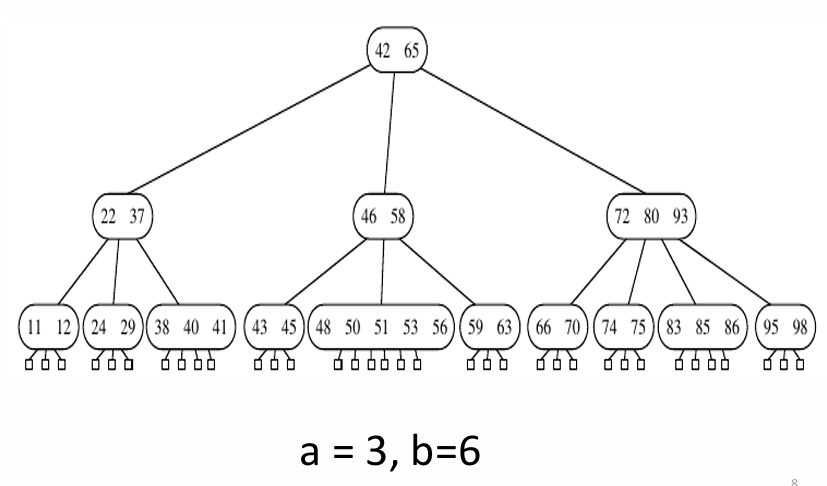
\includegraphics[width=0.47\linewidth]{Immagini/abTreeExample.png}
    \caption{a-b Tree}
\end{figure}

\subsubsection{Altezza di un abTree}
Considerando $n$ elementi memorizzati e sapendo che un albero di ricerca multi-way presenta sempre $n+1$ foglie, la struttura è vincolata dai seguenti parametri:
\begin{itemize}
    \item \textbf{Configurazione Minima (Worst Case)}: si verifica quando ogni nodo interno ha il numero minimo di figli ($a$). 
                                                       La radice ha $2$ figli e i livelli successivi si ramificano con fattore $a$, producendo un numero di foglie pari a $2a^{h-1}$.
    \item \textbf{Configurazione Massima (Best Case)}: Si verifica quando ogni nodo è saturo con $b$ figli. In questo scenario, il numero di foglie raggiunge il valore $b^h$. 
\end{itemize}

Questi vincoli si traducono nella disuguaglianza fondamentale $2a^{h-1} \le n+1 \le b^h$. Attraverso il calcolo logaritmico,
si isola la variabile dell'altezza ottenendo la relazione:$$(h-1)\log a + \log 2 \le \log(n+1) \le h \log b$$

Da questa derivazione si conclude che l'altezza $h$ è:
\begin{itemize}
    \item Limitata superiormente da $O(\log n / \log a)$.
    \item Limitata inferiormente da $\Omega(\log n / \log b)$.
\end{itemize}

In sintesi, l'uso di basi logaritmiche elevate ($a$ e $b$ grandi) permette di mantenere l'altezza estremamente ridotta, ottimizzando le prestazioni su grandi dataset.

\begin{figure}[H]
    \centering
    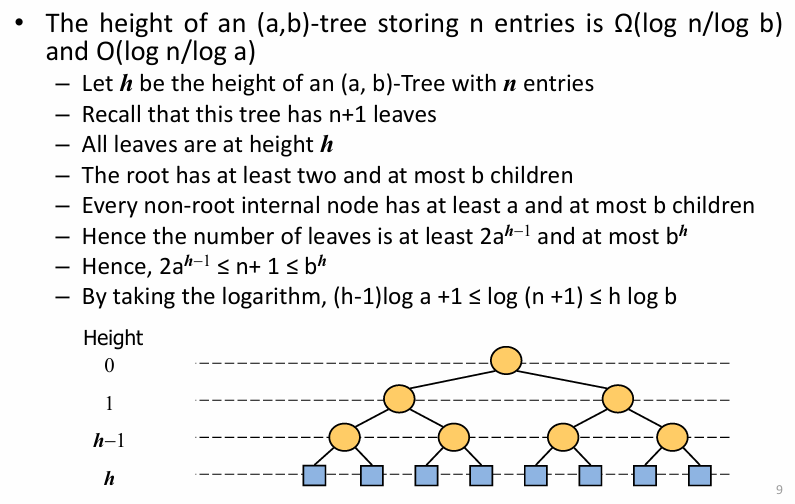
\includegraphics[width=0.47\linewidth]{Immagini/abTreeHeight.png}
    \caption{Altezza di un abTree}
\end{figure}

\subsubsection{Ricerca in un abTree}
\begin{figure}[H]
    \centering
    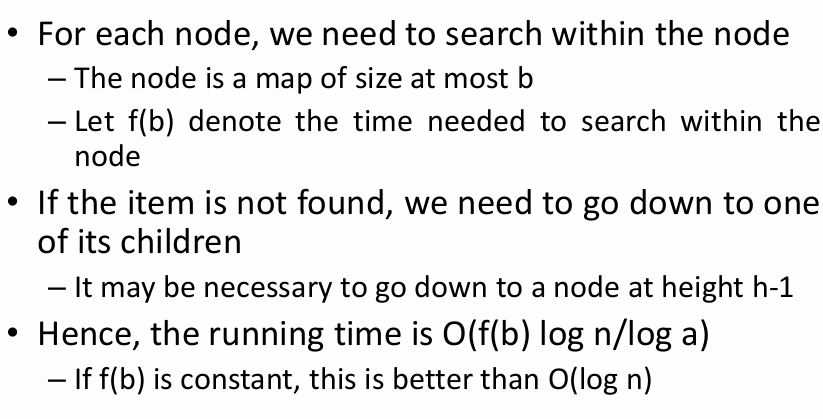
\includegraphics[width=0.47\linewidth]{Immagini/abTreeSearch.png}
    \caption{Ricerca in un abTree}
\end{figure}
\subsubsection{Inserimento in un abTree}
\begin{figure}[H]
    \centering
    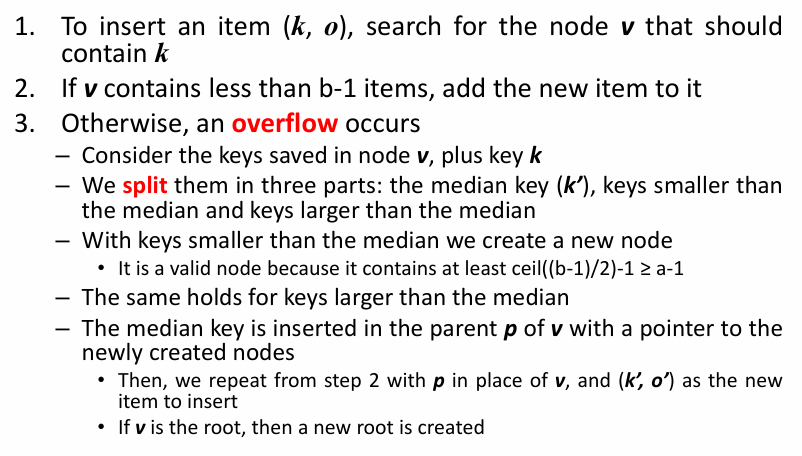
\includegraphics[width=0.47\linewidth]{Immagini/abTreeInsert.png}
    \caption{Inserimento in un abTree}
\end{figure}

\subsubsection{Cancellazione abTree}
\begin{figure}[H]
    \centering
    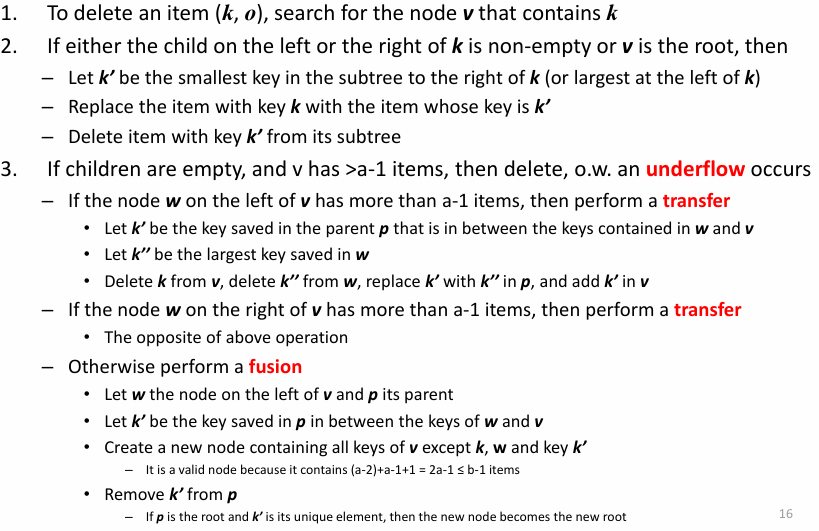
\includegraphics[width=0.47\linewidth]{Immagini/abTreeDelete.png}
    \caption{Cancellazione in un abTree}
\end{figure}

\subsection{B-tree}
\begin{figure}[H]
    \centering
    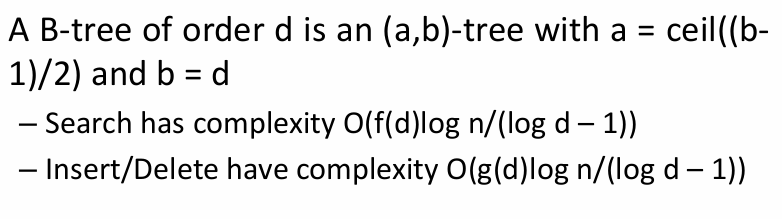
\includegraphics[width=0.47\linewidth]{Immagini/BTreeDef.png}
    \caption{B-tree}
\end{figure}

\subsection{Differenze tra MWST, ab-Tree, Btree}

\subsubsection{MWST}

Il Multiway Search Tree (il concetto base) è la definizione più libera.
Un nodo può avere un numero di figli $k$ qualsiasi. Se un nodo ha $k$ figli, contiene $k-1$ chiavi.
\begin{itemize}
    \item \textbf{Limiti}: Nessuno.  Non ci sono parametri $a$ o $b$ fissi.
    \item \textbf{Problema}: L'albero può diventare sbilanciato (molto alto e stretto), vanificando la velocità di ricerca.
\end{itemize}

\subsubsection{a-bTree}
Quando crei l'albero, fissi due numeri interi, $a$ e $b$. Una volta scelti, questi parametri non cambiano più per tutta la vita dell'albero.
\begin{itemize}
    \item \textbf{I Vincoli sui parametri}: per poter funzionare (e permettere lo split), devi scegliere $a$ e $b$ tali che:$$2 \le a \le \left\lceil \frac{b-1}{2} \right\rceil$$ \textit{Hint}: $\lceil3.4\rceil = 4$.
                                            \\Ad esempio, se fissi $b=10$, puoi scegliere un $a$ tra 2 e 5. Se scegli $a=2$, rimarrà 2 per sempre.
    \item \textbf{I Vincoli sui nodi}:  Ogni nodo interno deve avere un numero di figli $f$ compreso tra i parametri fissati: $a \le f \le b$.
    \item \textbf{Flessibilità}: È un modello teorico. Ti permette di decidere quanta "libertà" dare ai nodi (se $a$ è piccolo, i nodi possono essere quasi vuoti; se $a$ è vicino a $b/2$, i nodi devono essere più pieni).
\end{itemize}

\subsubsection{Btree}
Il B-Tree è un $(a, b)$-tree dove non hai libertà di scegliere $a$. Scegli solo il grado (o ordine) $d$, che corrisponde a $b$.

\begin{itemize}
    \item \textbf{I Parametri fissi}
    \begin{itemize}
        \item $b = d$
        \item $a = \lceil d-1/2 \rceil$
    \end{itemize}

    \item \textbf{La Filosofia}: Il B-Tree è "avaro" di spazio. Obbliga ogni nodo a essere pieno almeno al 50\%. Se un nodo scende sotto questa soglia (underflow), 
                                 l'albero si auto-ripara immediatamente tramite fusioni o prestiti.
\end{itemize}

\subsection{Quindi...}
Il MWST è la versione generale. Un nodo con $k$ chiavi ha $k+1$ figli.\\\\
L'a-bTree definisce dei limiti sul numero di figli di ogni nodo: 
\begin{itemize}
    \item \textbf{Numero massimo di figli}: $b$.
    \item \textbf{Numero minimo di figli}: $2\le a \le\left\lceil \frac{b-1}{2} \right\rceil$. 
\end{itemize}
\medskip
Il Btree è un a-bTree che impone il numero minimo al valore massimo consentito:
\begin{itemize}
    \item \textbf{Numero massimo di figli}: $b$.
    \item \textbf{Numero minimo di figli}: $a=\left\lceil \frac{b-1}{2} \right\rceil$. 
\end{itemize}
\medskip\medskip
Sotto il profilo dell'inserimento, le due strutture sono meccanicamente identiche: entrambe gestiscono l'eccesso di chiavi tramite lo \textit{split}.

\textbf{La vera differenza emerge nella \textit{Cancellazione}}\\
È qui che i due alberi si comportano diversamente:

\begin{itemize}
    \item Se in un $(a, b)$-tree con $a=2$ cancelli chiavi finché in un nodo ne resta solo una (2 figli), l'albero non fa nulla. Il nodo resta lì, mezzo vuoto.
    \item In un B-tree con $a=50$, appena scendi sotto le 49 chiavi (50 figli), l'albero "va nel panico".
          Deve attivare immediatamente operazioni di Merge (fusione) o Transfer (prestito da un vicino) per riportare il nodo sopra il 50\%.
\end{itemize}








\end{document}
